\section{RESULTS} \label{section:results}
We use Xeon E5-1650v4 to present the results of our optimization approach. Xeon E5-1650v4 has six cores where each core has 32 KB 8-way set associative L1 and 256 KB 8 way-set associative cache. They share a 15 MB 20-way set-associative cache.
\subsection{Machine Peak Overview}
Intel's micro-architecture specification indicates that the sustained L1 and L2 data cache bandwidth are $93$ bytes and $25$ bytes/cycle, respectively, whereas L3 bandwidth and DRAM
\begin{figure}[htbp]
\centerline{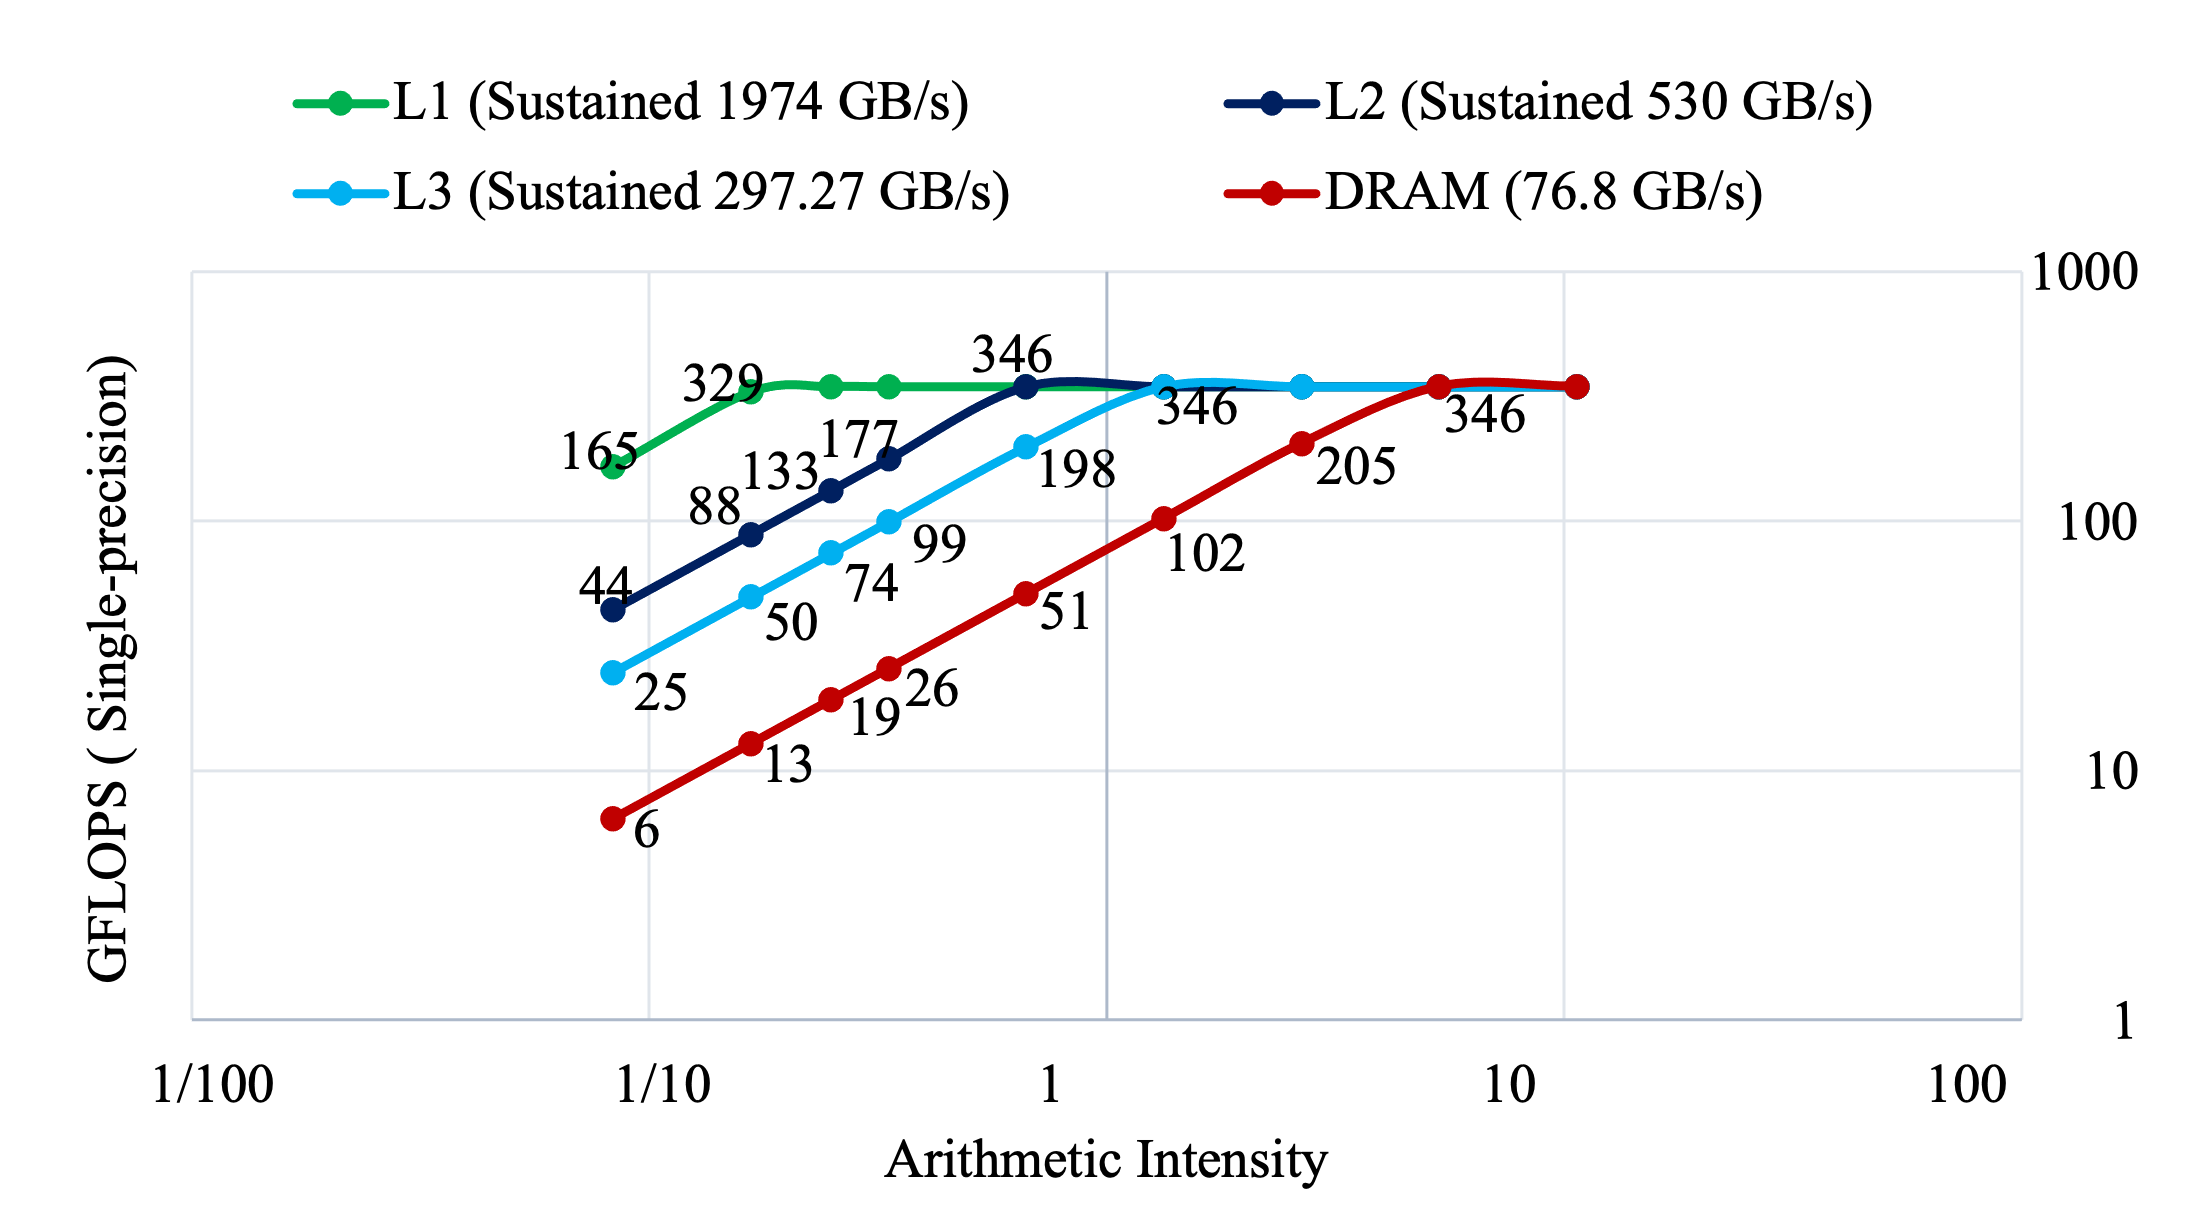
\includegraphics[scale=0.52, trim=5 5 5 5,clip]{figure_machine_roofline.png}}
\caption{Xeon E5 1650v4 roofline based on micro-architecture  }
%\caption{Xeon E5 1650v4 roofline based on micro-architecture  }
\label{fig:roof_line}
\end{figure}
bandwidth are $14$ bytes/cycle and $76.8$ GB/second,  respectively. Based on this data, we have come up with the roofline model shown in Figure~\ref{fig:roof_line}. The theoretical max-plus machine peak is about $346$ GFLOPS for single-precision. We will implicitly use GFLOPS to indicate the single-precision performance for the rest of the section. 
\begin{figure}[htbp]
\centerline{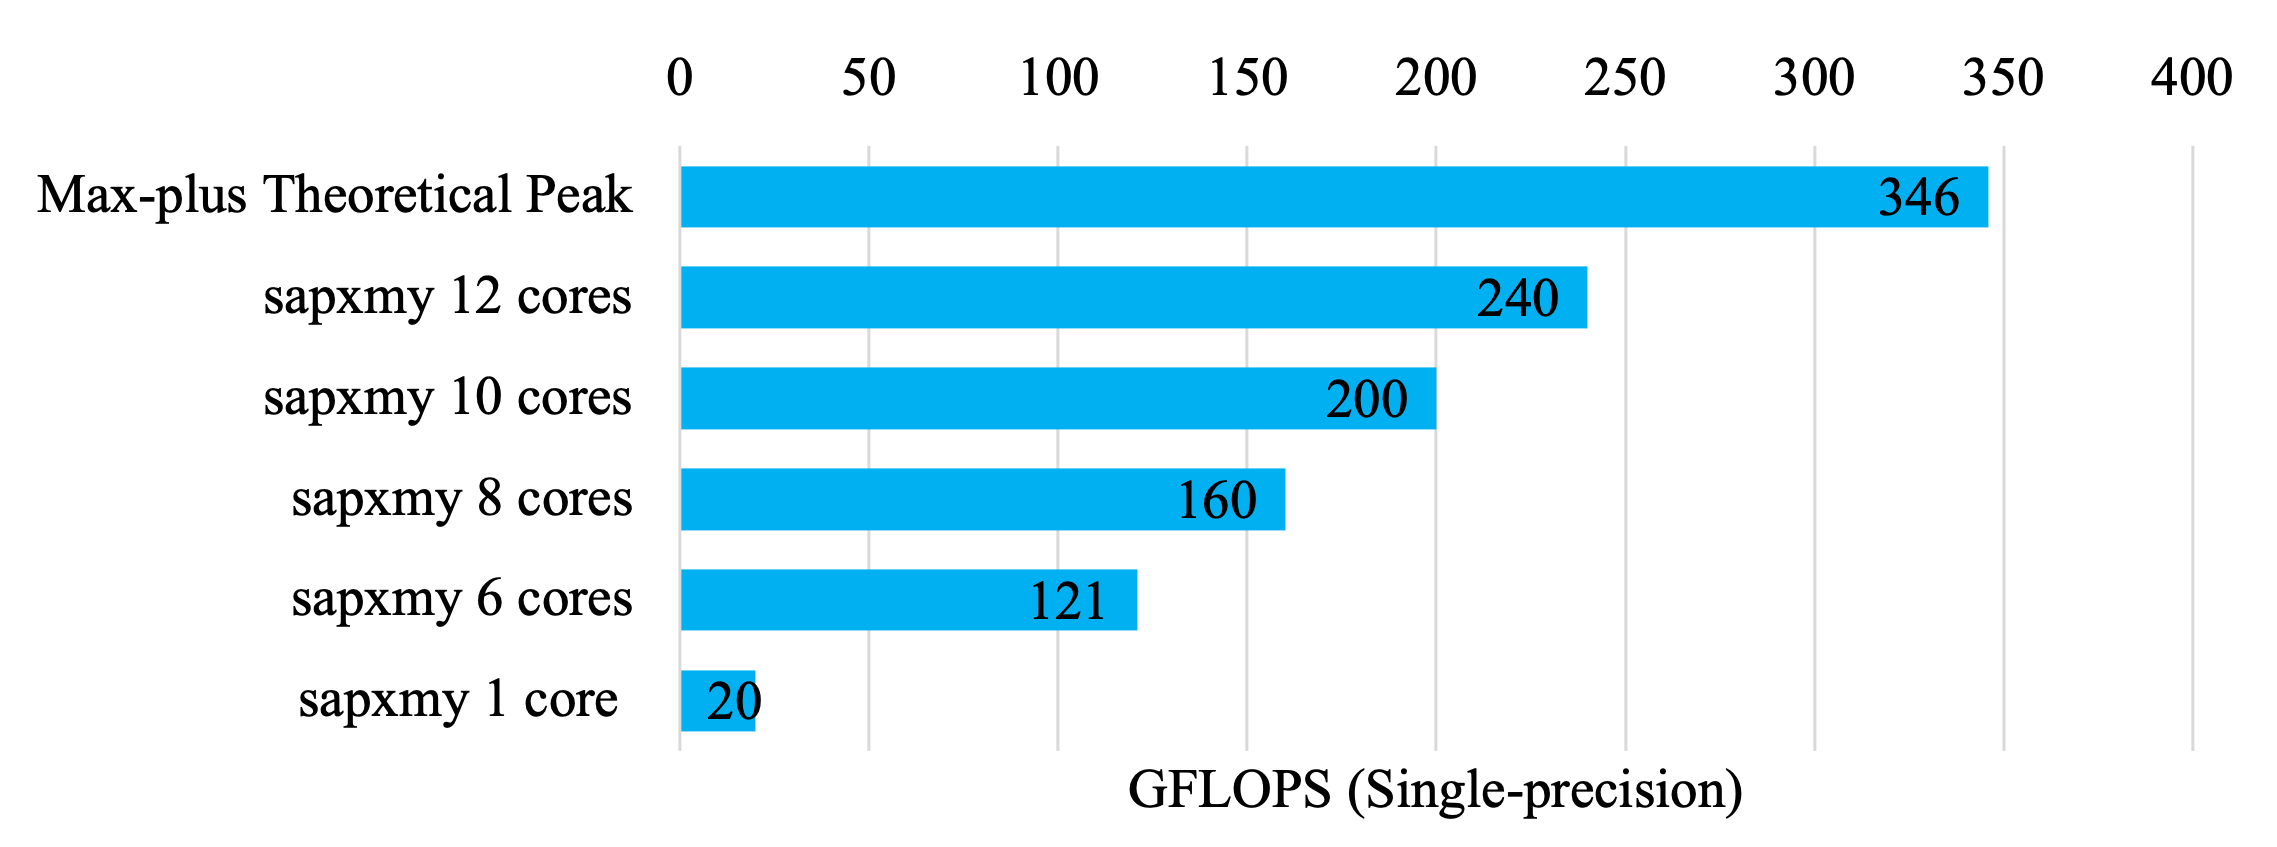
\includegraphics[scale=0.50, trim=5 5 5 5,clip]{figure_micro_benchmark.png}}
%\end{adjustbox}
\caption{Micro-benchmark for $Y= \max(a+X, Y)$}
\label{fig:micro_bench_mark}
\end{figure}
BPMax performs 2-arithmetic operations for 3-single-precision memory operations. So, its arithmetic intensity is $\frac{2}{(3 \times 4)}$ or $ \frac{1}{6}$ (second data points on each series shown in Figure~\ref{fig:roof_line}). Based on the roofline model, we expect to achieve around $329$ GFLOPS based on L1 bandwidth. Our micro-benchmark data (Figure~\ref{fig:micro_bench_mark}) shows that we achieve up to $120$ GFLOPS with $6$ threads and $240$ GFLOPS with $12$ threads.

\subsection{Performance Analysis of Double Max-plus Computation}
In this section, we go over the results of our optimization approach for double max-plus computation. Figure~\ref{fig:peroformance_analysis_double_max_plus} and  Figure~\ref{fig:double_max_plus_speed_up} show the performance and speedup comparison of double max-plus between different schedules using $6$ threads.  We see that the coarse-grain parallelization performs very poorly since it generates a lot of DRAM traffic and makes the program slower. There is a minor difference between computing the inner triangles of $F$-table diagonally vs. bottom-up and left to right highlighted in orange and blue. In both cases, all the threads work on one inner triangle before moving to the next. Our tiling approach improves locality and maintains automatic vectorization. It enables us to get close to the $97\%$ of our micro-benchmark target. We attain $117$ GFLOPS with the tiling transformation. Tile dimensions of $(32 \times 4 \times N)$ and $(64 \times 16 \times N)$ are used for presenting the performance and speedup comparison. $(32 \times 4 \times N)$ is restricted for sequence length up to 2048. 

We achieve around $178\times$ improvement over the base implementation taken from the BPMax program. It is a sequential improvement of $40-200\%$ with $6$ threads over Varadrajan’s fine-grain schedule. However, her results show that hyperthreading helped improve performance by over $10\%$ in some cases. We see minimal ($3-5\%$) improvement with hyper-threading over six threads shown in Figure~\ref{fig:hyperthreading_effect}. We have done experiments with different tile sizes ($ i_{2} \times k_{2} \times j_{2}$) and found that the cubic tiles perform poorly. We observe the best result when  $j_{2}$ is not tiled due to the streaming effect. 
\begin{figure*}[htbp]
\centerline{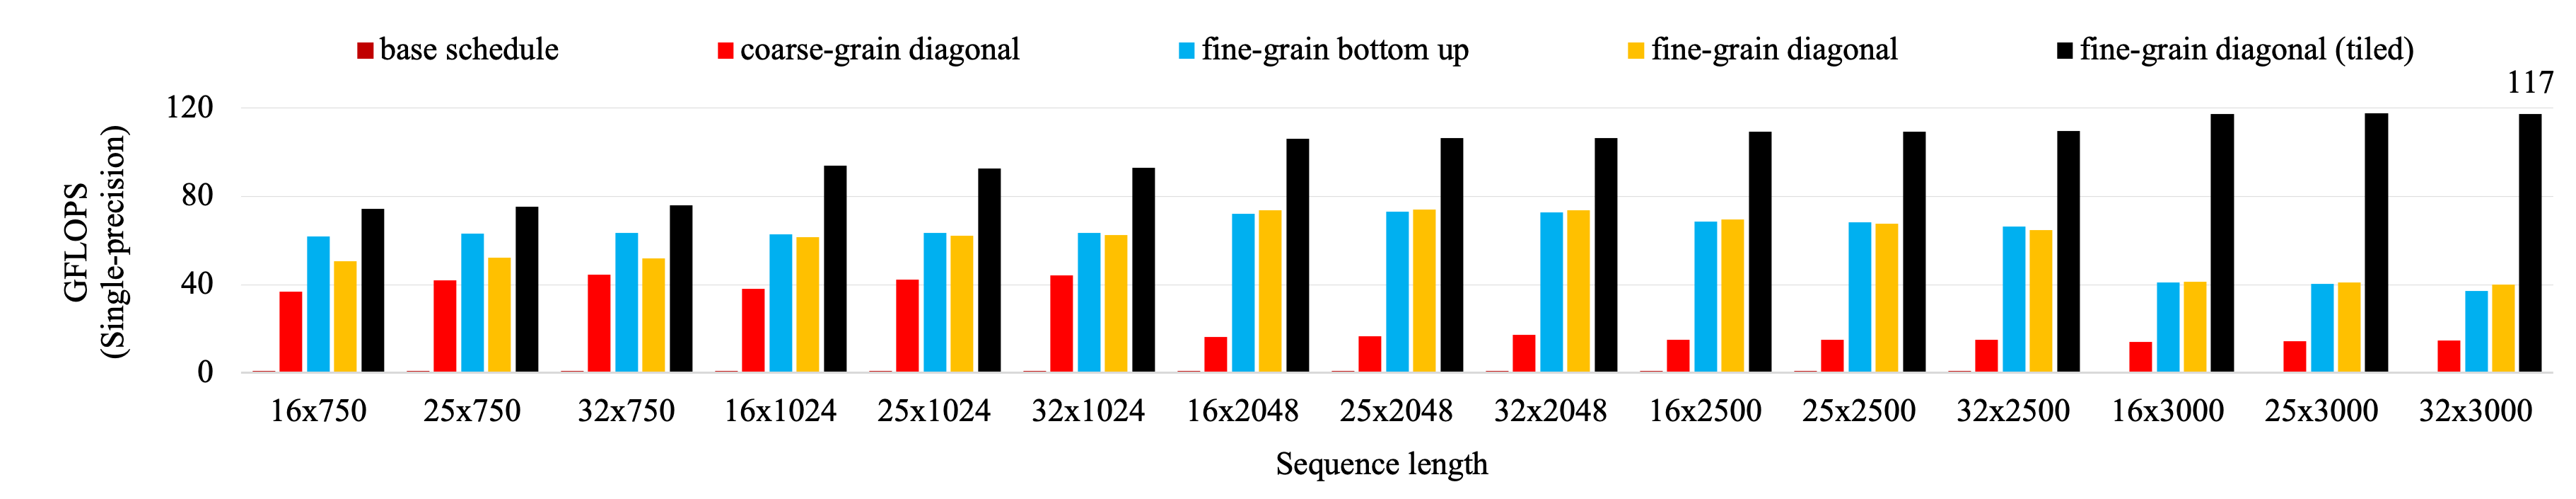
\includegraphics[width=\textwidth,scale=1.00, trim=5 5 5 5,clip]{dmp_performance_new.png}}
\caption{Double max-plus performance comparison}
\label{fig:peroformance_analysis_double_max_plus}
\end{figure*}

\begin{figure*}[htbp]
 \centerline{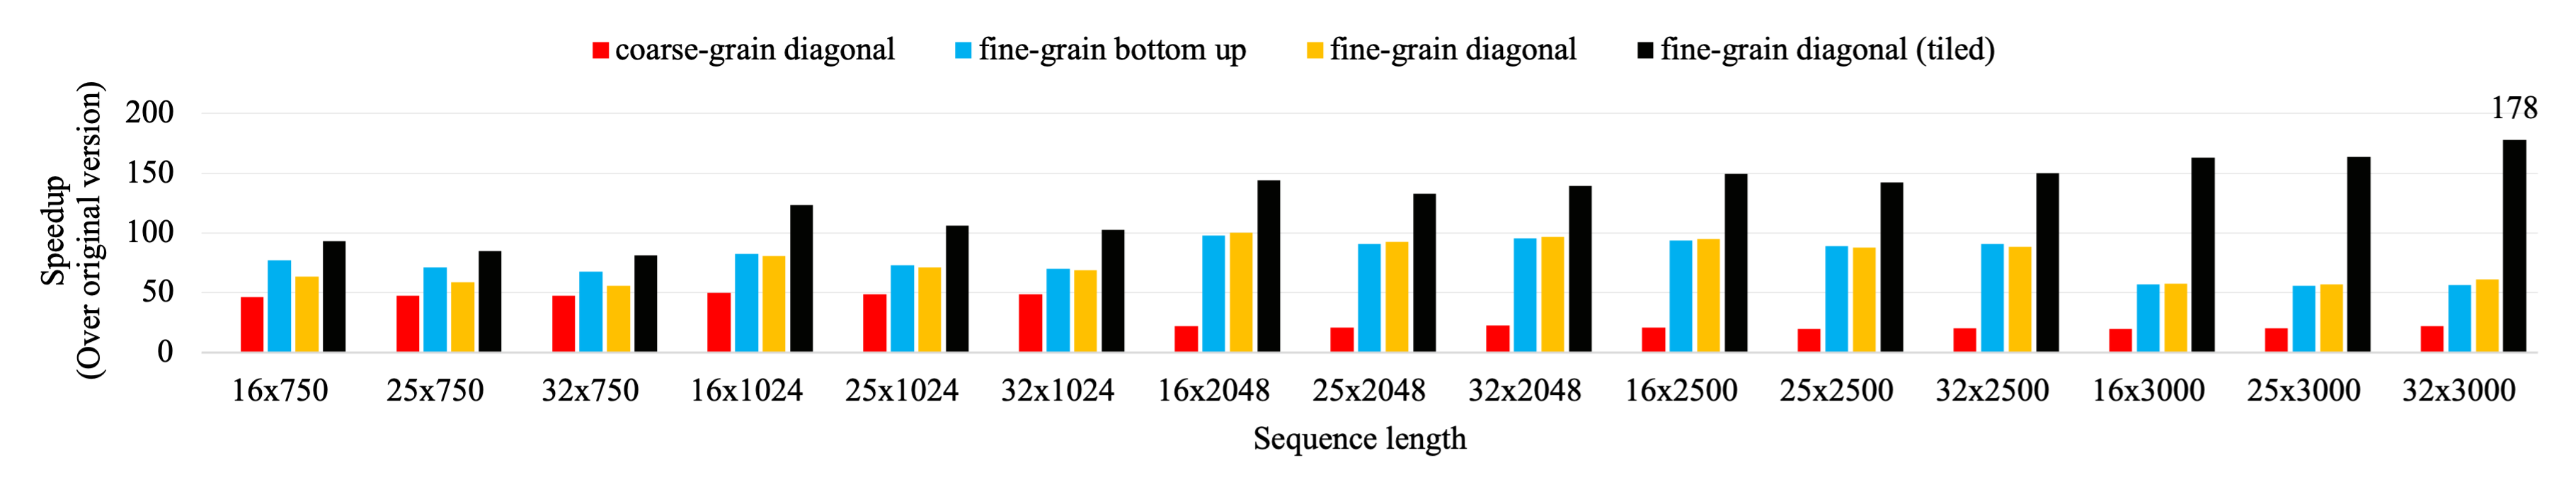
\includegraphics[width=\textwidth,scale=1.00, trim=5 5 5 5,clip]{dpm_speed_up_new.png}} 
%\end{adjustbox}
\caption{Double max-plus speedup comparison}
\label{fig:double_max_plus_speed_up}
\end{figure*}


\begin{figure*}[htbp]
\centerline{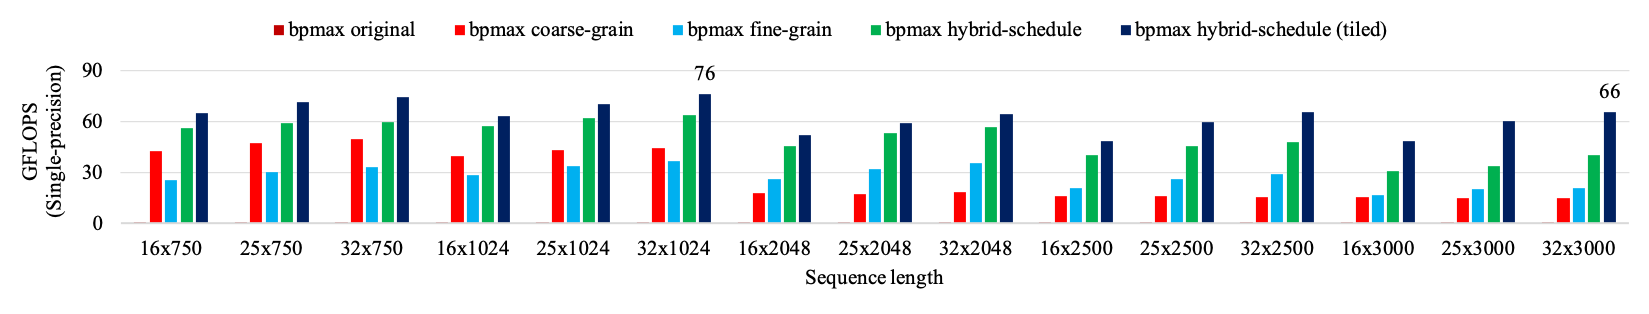
\includegraphics[width=\textwidth,scale=1.00, trim=5 5 5 5,clip]{bpm_performance_new.png}} 
\caption{BPMax performance comparison}
\label{fig:bpm_performance}
\end{figure*}

\begin{figure*}[htbp]
\centerline{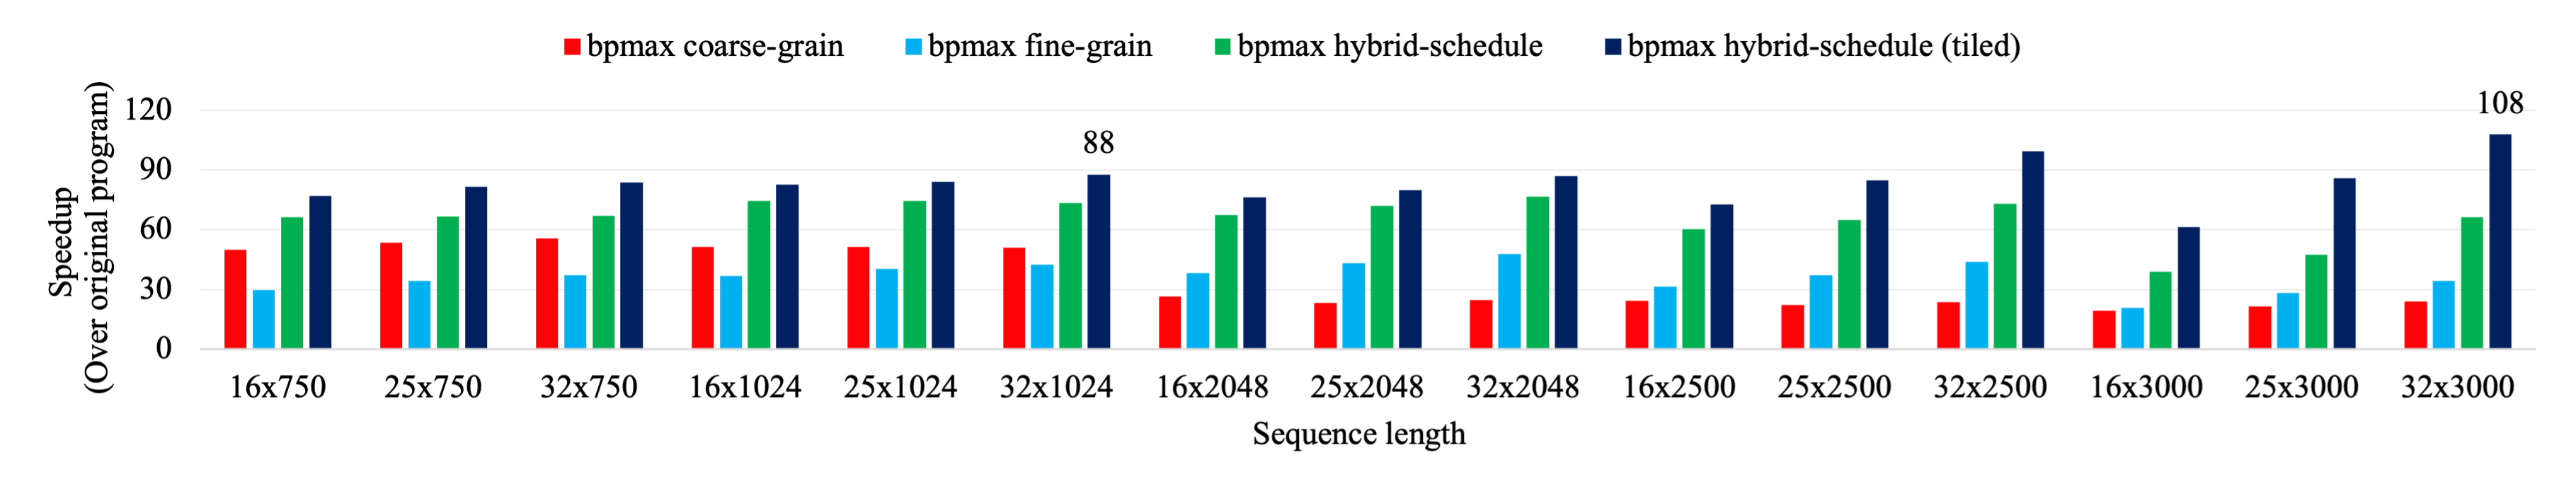
\includegraphics[width=\textwidth,scale=1.00, trim=5 5 5 5,clip]{bpm_speed_up_new.png}} 
\caption{BPMax speedup comparison}
\label{fig:bpm_speed_up}
\end{figure*}

%\begin{figure*}[!t]
%\centering
%\begin{subfigure}[t]{0.48\linewidth}
%\centering
%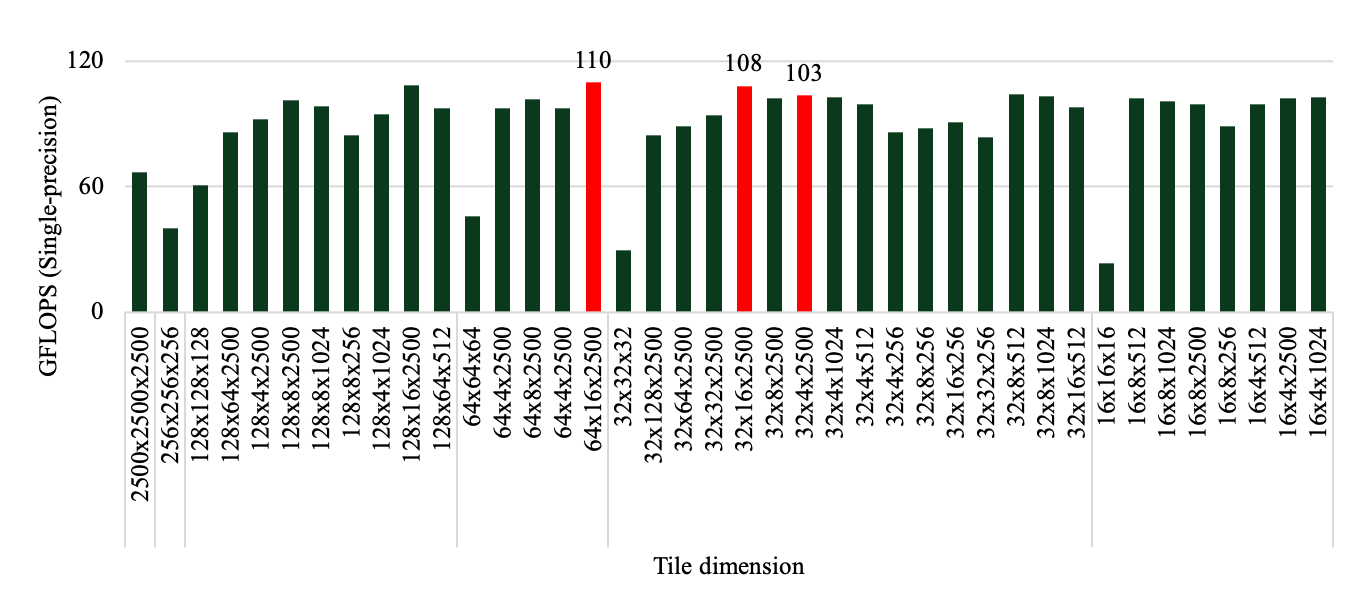
\includegraphics[scale=0.38, trim=5 5 5 5,clip]{double_max_plus_tile_exploration.png}
%\caption{Effect of tiling parameters ($i_{2} \times k_{2} \times j_{2}$) on double max-plus performance  - sequence length 16 x 2500}
%%\label{fig:tiling_parameter}
%\end{subfigure}
%\begin{subfigure}[t]{0.48\linewidth}
%\centering
%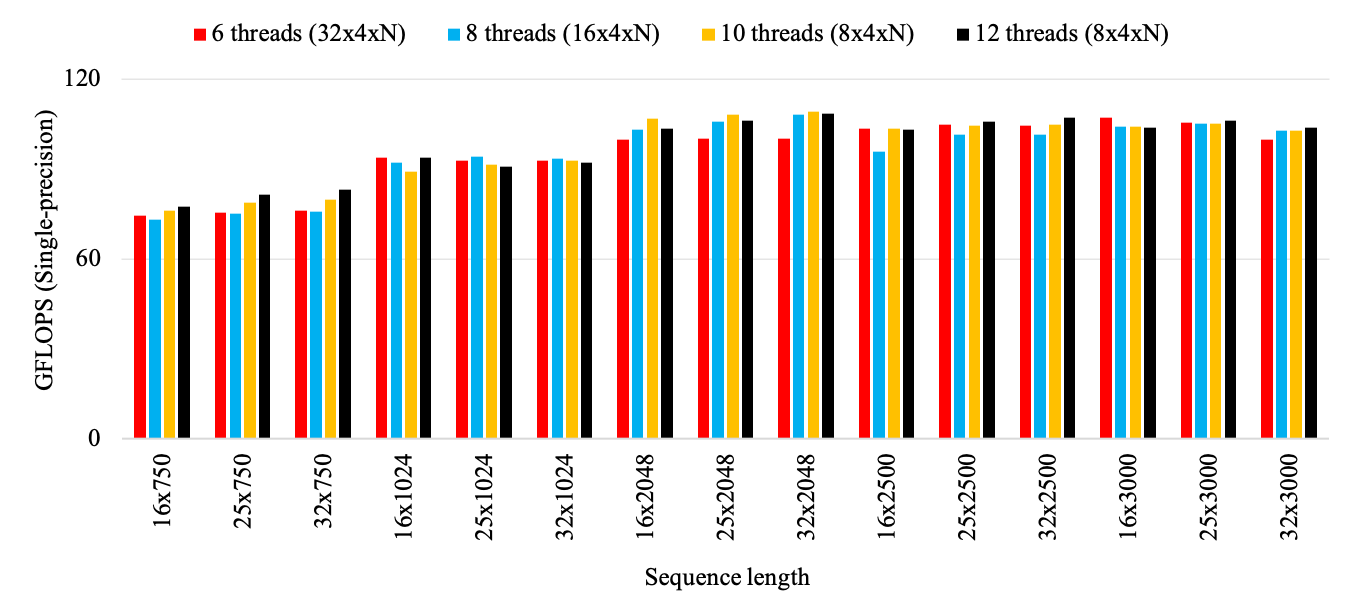
\includegraphics[scale=0.48, trim=5 5 5 5,clip]{double_max_plus_hyperthreading_new.png}
%\caption{Effect of hyper-threading on tiled double max-plus performance}
%\label{fig:hyperthreading_effect}
%\end{subfigure}
%\end{figure*}

\begin{figure}[htbp]
\centerline{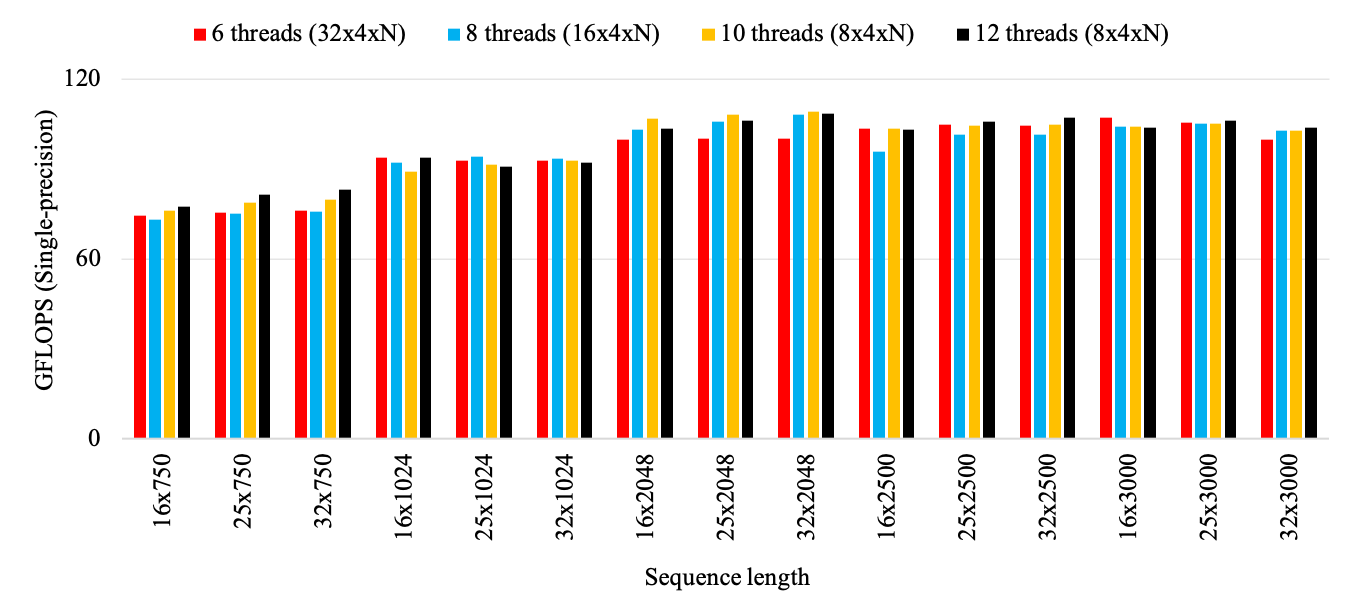
\includegraphics[scale=0.40, trim=4 4 4 4,clip]{double_max_plus_hyperthreading_new.png}}
\caption{Effect of hyper-threading on tiled double max-plus performance}
\label{fig:hyperthreading_effect}
\end{figure}

\begin{figure}[htbp]
\centerline{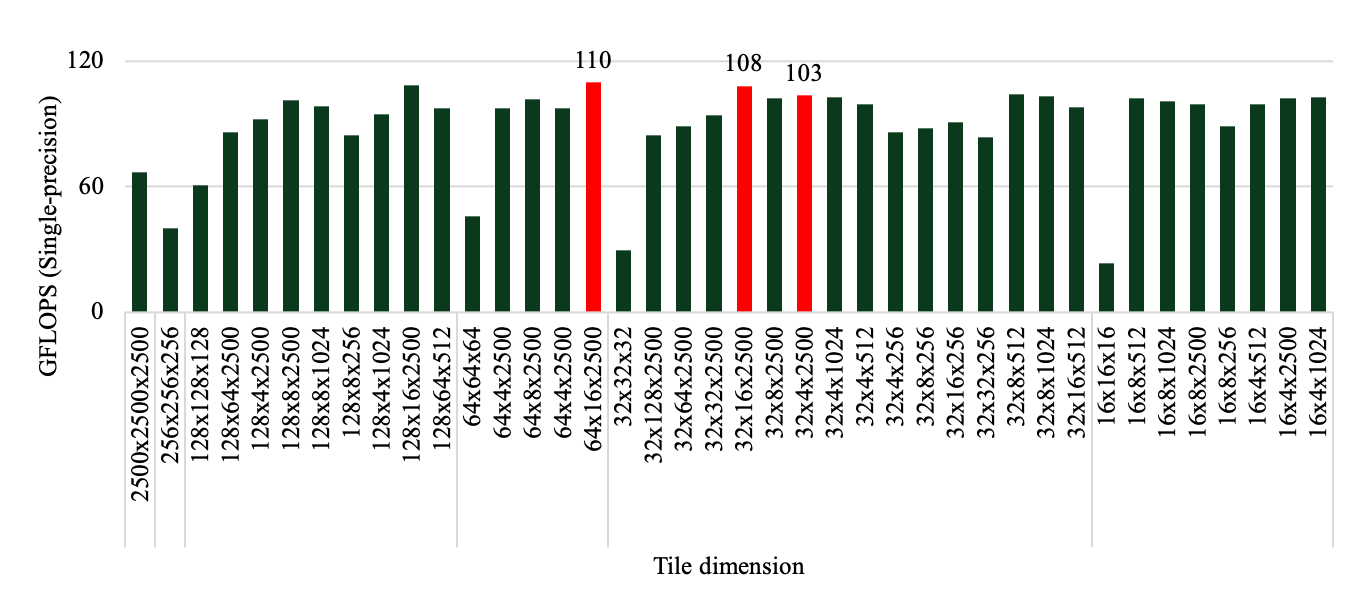
\includegraphics[scale=0.40, trim=4 4 4 4,clip]{double_max_plus_tile_exploration.png}}
\caption{Effect of tiling parameters ($i_{2} \times k_{2} \times j_{2}$) on double max-plus performance (sequence length - 16 x 2500)}
\label{fig:tiling_parameter}
\end{figure}


\subsection{BPMax  Performance Improvement}
Figure~\ref{fig:bpm_performance} and ~\ref{fig:bpm_speed_up} show the performance improvements and speedup  of different versions of the BPMax program using $6$ threads. We use the original BPMax program as the reference since no better CPU-version of the BPMax program is available. The coarse and fine-grain version of the program performs the worst, highlighted in light red and blue. As seen in the previous section, the coarse-grain schedule severely impacts double max-plus computation, affecting overall performance. Fine-grain parallelism works better for $R_0$, $R_3$, $R_4$, but we cannot parallelize the $R_1$, and $R_2$ computations. The hybrid parallelization approach highlighted in green performs better than the coarse and fine-grain schedule. The tiled version of the hybrid schedule highlighted in dark blue performs best. It achieves $100\times$ speedup for longer sequence lengths with $6$ threads. The improvement for the tiled version mainly comes from the optimization of $R_0$, $R_3$, $R_4$. The tiled version of the program reaches around $76$ GFLOPS for moderate-size sequences. It is almost $60\%$ lower than the best double max-plus version of the same sequence. Our analysis shows that $R_3$ and $R_4$ are almost free since those get computed along with the $R_0$. The other two $\Theta(M^2N^3)$ computations - $R_{1}$ and $R_{2}$ severely affect the overall performance. It is the effect of our schedule choice. Each thread is responsible for producing the final version of one inner triangle of $F$-table along with the $R_{1}$ and $R_{2}$. Both of these computations require most of the elements of one inner triangle of $F$-table and the $S^{(2)}$-table to compute one row for the worst case. So, the total amount of data required to process a row reaches about $\Theta(N^2)$, which is $16$ MB for an inner sequence of length $2048$. This issue gets amplified when we attempt hyper-threading (beyond $6$ threads for E5-1650v4).  

%Besides Xeon E5-1650v4, we have verified that the performance of the optimized BPMax scales up on Intel Xeon E-2278G, which has eight cores. Figure~\ref{fig:bpm_quick_compare} shows an overview of the performance and speedup comparison on Xeon E-2278G  and Xeon E5-1650v4.
%We have tried to adjust the degree of parallelism to smaller than the number of physical cores for  $R_{1}$ and $R_{2}$. 

Besides Xeon E5-1650v4, we have verified the scalability of our optimized program on Intel Xeon E-2278G, which has eight cores and runs almost at the same speed as E5-1650v4. The optimized BPMax performs the same or better on  E-2278G compare to E5-1650v4, reaching close to one-fourth of the theoretical single-precision machine peak. Figure~\ref{fig:bpm_quick_compare} shows an overview of the performance and speedup comparison on Xeon E-2278G  and Xeon E5-1650v4.

\subsection{Code Generation Metric}

Table~\ref{tab1:codegen_metric} shows the line of code (\textit{LOC}) generated by \alphaz\ for different BPMax program versions. We see an increase in \textit{LOC}  when the program is optimized. Also, the table highlights the complexities (based on \textit{LOC}) between the double max-plus computation and the BPMax program.

\begin{table}[htbp]
\caption{\uppercase{Auto-generated code statistics}}
\begin{center}
\begin{tabular}{|c|c|c|c|}
\hline
\textbf{\textit{Implementation}}& {\textit{LOC}} & \textbf{\textit{${\mathrm{a}}$}} & \textbf{\textit{${\mathrm{b}}$}} \\
\hline
BPMax base  & 140 & 140 & NA   \\
\hline
Double max-plus(coarse/fine)  & 150 & None & 3   \\
\hline
BPMax coarse/fine/ hybrid & 1200 & None & 30  \\
\hline
BPMax hybrid with tiled & 1400 & $<$5 & 7   \\
\hline
\multicolumn{3}{l}{${\mathrm{a}}$ - Hand written code}\\
\multicolumn{3}{l}{${\mathrm{b}}$ - Macro replacement/Macro comment out}\\
\end{tabular}
\label{tab1:codegen_metric}
\end{center}
\end{table}

